\hypertarget{test}{%
\section{Test}\label{test}}

In this application different aspects will be tested.

\hypertarget{ltsa-model}{%
\subsection{LTSA model}\label{ltsa-model}}

The LTSA model will using the LTSA desgin tool safety, progress and
supertrace tests.

\hypertarget{safety}{%
\subsubsection{Safety}\label{safety}}

Using the safety test of LTSA design tool the following output is
produced:

\begin{figure}
\centering
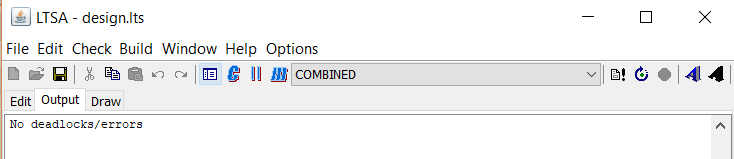
\includegraphics{../img/safety.png}
\caption{Safety test}
\end{figure}

\hypertarget{progress}{%
\subsubsection{Progress}\label{progress}}

Using the progress test of LTSA design tool the following output is
produced:

\begin{figure}
\centering
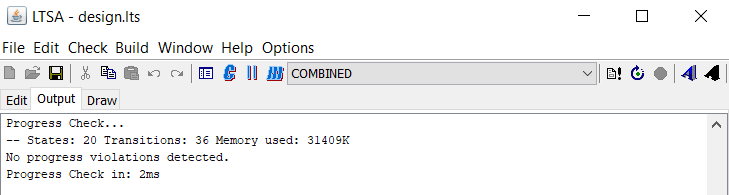
\includegraphics{../img/progress.png}
\caption{Progress test}
\end{figure}

\hypertarget{supertrace}{%
\subsubsection{Supertrace}\label{supertrace}}

Using the supertrace test of LTSA design tool the following output is
produced:

\begin{figure}
\centering
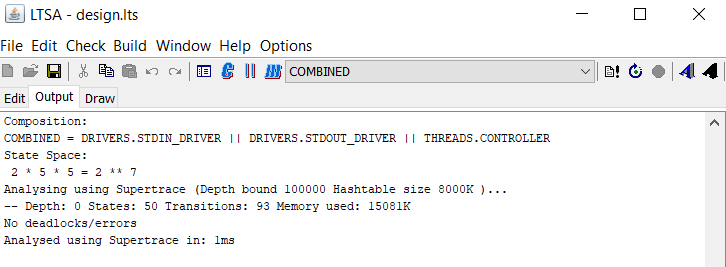
\includegraphics{../img/supertrace.png}
\caption{Supertrace test}
\end{figure}

\hypertarget{the-minix-implementation}{%
\subsection{The minix implementation}\label{the-minix-implementation}}

When running the implementation on Minix it produces the following
output:

\begin{figure}
\centering
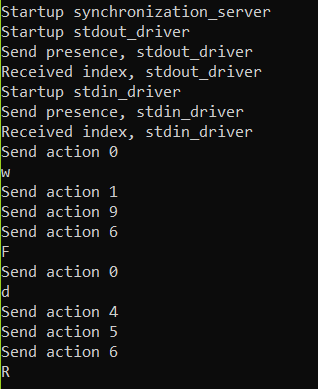
\includegraphics{../img/output.png}
\caption{Minix run test}
\end{figure}

Here the character `w' and `d' where read from the input line. This
output is one of the possible traces that can be followed from the FSP
model, and was tested in LTSA tools:

\begin{figure}
\centering
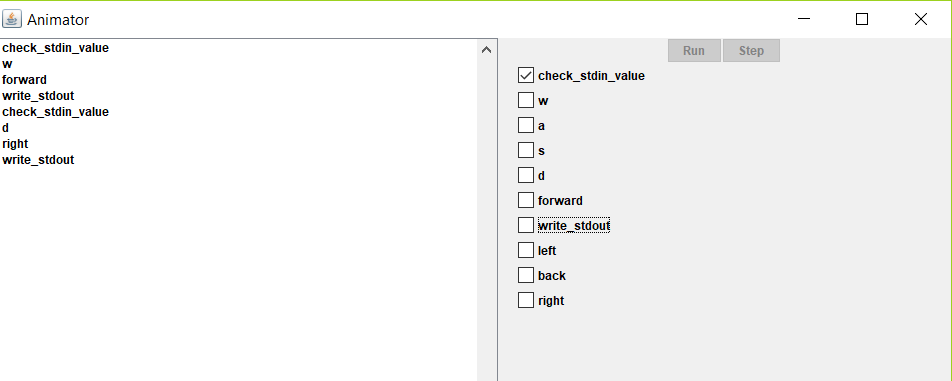
\includegraphics{../img/ltsa_output.png}
\caption{LTSA tool trace}
\end{figure}

This concludes that the application build can follow from an FSP design,
as this was the aim of this paper.
